\documentclass[../Main.tex]{subfiles}
\begin{document}
Given the distinctive characteristics of the system discussed in Chapter 3, it is essential to adopt an architecture or combination of multiple architectures to efficiently address these specific requirements while ensuring scalability, reliability, and seamless communication between different components. This chapter aims to deliver an in-depth exploration of the architecture design implemented in the project and provide a detailed understanding of each element in the system.
\section{Architecture design}
\subsection{Software architecture selection}
\begin{figure}[H]
    \centering
    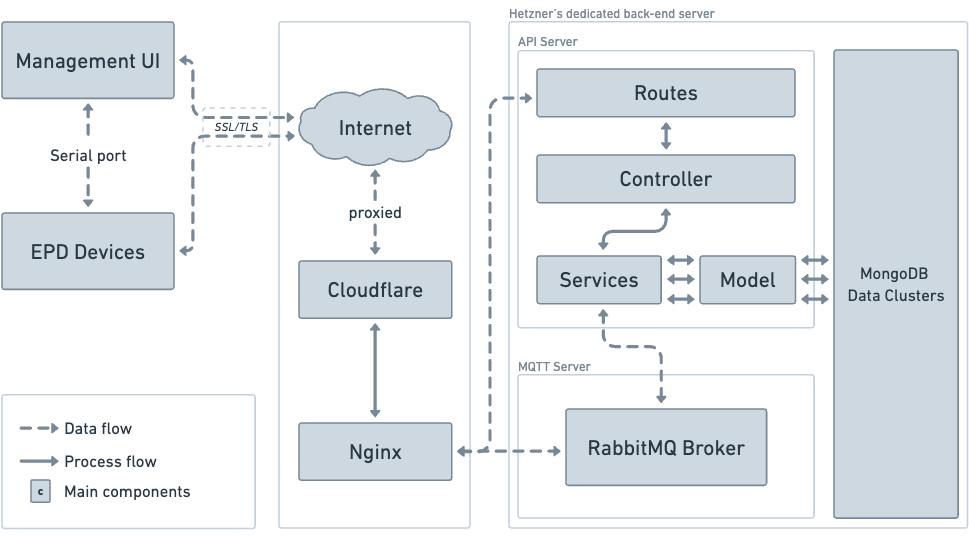
\includegraphics[scale=0.46]{doc/thesis/EN/imgs/overall-architecture.png}
    \caption{Overall architecture of the system}
    \label{fig:Fig1}
\end{figure}

\textbf{Figure \ref{fig:Fig1}} illustrates the system's general architecture and provides an overview of its data flow. The system strategically uses the combination of MVCS (Model-View-Controller-Service) and microservice architectures to take advantage of their unique strengths in specific aspects. This hybrid architecture leverages the benefits of both architectural styles, such as scalability, flexibility, and the ability to use different technologies and patterns within each service.

Microservices architecture is a software development method that structures an application as a collection of loosely coupled services. In this architecture, each service can be developed, deployed, and scaled independently, allowing greater scalability, flexibility, and agility than monolithic architectures, as teams can update or fix individual components without impacting the entire system in case of failure. Thanks to its ability to accommodate the dynamic and distributed natures of IoT applications, microservice architecture is frequently used in various IoT projects. It allows organizations to build more agile and adaptive applications to handle the complex demands of modern business environments.

On the other hand, the Model-View-Controller-Service (MVCS) architecture is an extension of the traditional Model-View-Controller (MVC) pattern. It introduces a service layer sitting between the controller and the model, which is responsible for containing business logic and rules. This layer abstracts complex business operations, allowing Controllers to focus on handling incoming requests and delegating the heavy lifting to Services. This design pattern is well-suited to many web applications and provides a structured and organized approach to developing complex applications, making it easier to manage, maintain, and scale the system over time.

By combining these two architectures, the system is better equipped to handle the dynamic and distributed nature of IoT applications. It also enables organizations to build more agile and adaptive applications to address the complex demands of modern business environments while ensuring scalability, reliability, and seamless communication between different components.

\subsection{Overall design}
The system is divided into independently deployable services, including the API back-end server and MQTT Server. These services communicate via the MQTT protocol, and the MQTT Server also acts as a broker to relay data to the EPD devices (Figure \ref{fig:Fig3}). API server follows the MVCS pattern with three main components: Controllers handling incoming requests and coordinating responses, Services containing the business logic and rules of the application, and Models interacting with the database, managing data storage and retrieval, while Management UI and EPD devices act as a View component (Figure \ref{fig:Fig2}).
\subsubsection{MVCS architecture}
The system has three data types, and the packages of each type handling operation share the same structure: the Controller handles requests about the data type and delegates them to the Service, which processes the requests and uses the Model to interact with the database.
\begin{figure}[H]
    \centering
    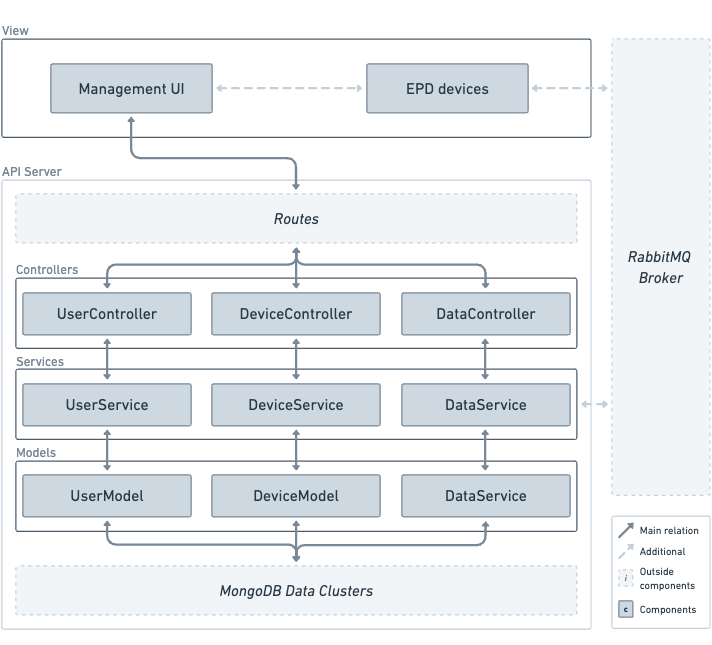
\includegraphics[scale=0.6]{doc/thesis/EN/imgs/api-server.png}
    \caption{MVCS architecture}
    \label{fig:Fig2}
\end{figure}

\subsubsection{MQTT Server}
This service in the system acts as an intermediary, managing the state of all MQTT client connections, subscriptions, and message exchanges.
\begin{figure}[H]
    \centering
    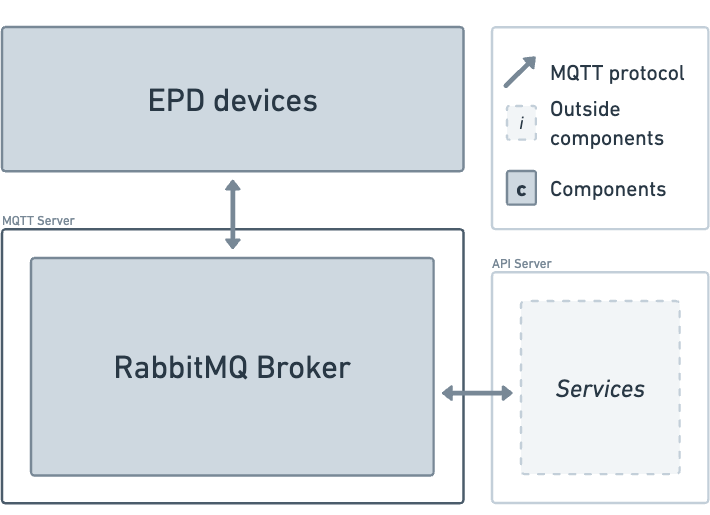
\includegraphics[scale=0.3]{doc/thesis/EN/imgs/mqtt-server.png}
    \caption{MQTT microservice}
    \label{fig:Fig3}
\end{figure}

\subsection{Detailed package design}
Sinh viên thiết kế và lần lượt vẽ biểu đồ thiết kế cho từng package, hoặc một nhóm các package liên quan để giải quyết một vấn đề gì đó. Khi vẽ thiết kế gói, sinh viên chỉ cần đưa tên lớp, không cần chỉ ra các thành viên phương thức và thuộc tính. SV tham khảo ví dụ minh họa trong Hình \ref{fig:Fig2}.

Sinh viên cần vẽ rõ ràng quan hệ giữa các lớp trong biểu đồ. Các quan hệ bao gồm: phụ thuộc (dependency), kết hợp (association), kết tập (aggregation), hợp thành (composition), kế thừa (inheritance), và thực thi (implementation). Các quan hệ này đều đã được minh họa trong \ref{fig:Fig2}.

\section{Detailed design}
\subsection{User interface design}
Phần này có độ dài từ hai đến ba trang. Sinh viên đặc tả thông tin về màn hình mà ứng dụng của mình hướng tới, bao gồm độ phân giải màn hình, kích thước màn hình, số lượng màu sắc hỗ trợ, v.v. Tiếp đến, sinh viên đưa ra các thống nhất/chuẩn hóa của mình khi thiết kế giao diện như thiết kế nút, điều khiển, vị trí hiển thị thông điệp phản hồi, phối màu, v.v. Sau cùng sinh viên đưa ra một số hình ảnh minh họa thiết kế giao diện cho các chức năng quan trọng nhất. Lưu ý, sinh viên không nhầm lẫn giao diện thiết kế với giao diện của sản phẩm sau cùng.
\subsection{Layer design}
Phần này có độ dài từ ba đến bốn trang. Sinh viên trình bày thiết kế chi tiết các thuộc tính và phương thức cho một số lớp chủ đạo/quan trọng nhất của ứng dụng (từ 2-4 lớp). Thiết kế chi tiết cho các lớp khác, nếu muốn trình bày, sinh viên đưa vào phần phụ lục.

Để minh họa thiết kế lớp, sinh viên thiết kế luồng truyền thông điệp giữa các đối tượng tham gia cho 2 đến 3 use case quan trọng nào đó bằng biểu đồ trình tự (hoặc biểu đồ giao tiếp).
\subsection{Database design}
Phần này có độ dài từ hai đến bốn trang. Sinh viên thiết kế, vẽ và giải thích biểu đồ thực thể liên kết (E-R diagram). Từ đó, sinh viên thiết kế cơ sở dữ liệu tùy theo hệ quản trị cơ sở dữ liệu mà mình sử dụng (SQL, NoSQL, Firebase, v.v.)

\section{Application Building}
\subsection{Libraries and Tools}
Sinh viên liệt kê các công cụ, ngôn ngữ lập trình, API, thư viện, IDE, công cụ kiểm thử, v.v. mà mình sử dụng để phát triển ứng dụng. Mỗi công cụ phải được chỉ rõ phiên bản sử dụng. SV nên kẻ bảng mô tả tương tự như Bảng \ref{table:my_label}. Nếu có nhiều nội dung trình bày, sinh viên cần xoay ngang bảng.

\begin{table}[H]
\centering{}
    \begin{tabular}{lll}
        \hline
        \textbf{Mục đích} & \textbf{Công cụ}       & \textbf{Địa chỉ URL}    \\ \hline
        IDE lập trình     & Eclipse Oxygen a64 bit & http://www.eclipse.org/ \\ \hline
        v.v.              & v.v.                   & v.v.                    \\ \hline
        \end{tabular}
    \caption{Danh sách thư viện và công cụ sử dụng}
    \label{fig:my_label}
\end{table}

\subsection{Achievement}
Sinh viên trước tiên mô tả kết quả đạt được của mình là gì, ví dụ như các sản phẩm được đóng gói là gì, bao gồm những thành phần nào, ý nghĩa, vai trò?

Sinh viên cần thống kê các thông tin về ứng dụng của mình như: số dòng code, số lớp, số gói, dung lượng toàn bộ mã nguồn, dung lượng của từng sản phẩm đóng gói, v.v. Tương tự như phần liệt kê về công cụ sử dụng, sinh viên cũng nên dùng bảng để mô tả phần thông tin thống kê này.

\subsection{Illustration of main functions}
Sinh viên lựa chọn và đưa ra màn hình cho các chức năng chính, quan trọng, và thú vị nhất. Mỗi giao diện cần phải có lời giải thích ngắn gọn. Khi giải thích, sinh viên có thể kết hợp với các chú thích ở trong hình ảnh giao diện.

\section{Testing}
Phần này có độ dài từ hai đến ba trang. Sinh viên thiết kế các trường hợp kiểm thử cho hai đến ba chức năng quan trọng nhất. Sinh viên cần chỉ rõ các kỹ thuật kiểm thử đã sử dụng. Chi tiết các trường hợp kiểm thử khác, nếu muốn trình bày, sinh viên đưa vào phần phụ lục.
Sinh viên sau cùng tổng kết về số lượng các trường hợp kiểm thử và kết quả kiểm thử. Sinh viên cần phân tích lý do nếu kết quả kiểm thử không đạt.
\section{Deployment}
Sinh viên trình bày mô hình và/hoặc cách thức triển khai thử nghiệm/thực tế. Ứng dụng của sinh viên được triển khai trên server/thiết bị gì, cấu hình như thế nào. Kết quả triển khai thử nghiệm nếu có (số lượng người dùng, số lượng truy cập, thời gian phản hồi, phản hồi người dùng, khả năng chịu tải, các thống kê, v.v.)

\end{document}
